\documentclass[onecolumn, draftclsnofoot,10pt, compsoc]{IEEEtran}
\usepackage{graphicx}
\usepackage{url}
\usepackage{pgfgantt}
\usepackage{minted}
\usepackage{setspace}
\usepackage{geometry}
\geometry{textheight=9.5in, textwidth=7in}

% 1. Fill in these details
\def \CapstoneTeamName{		The Seed Team}
\def \CapstoneTeamNumber{		32}
\def \GroupMemberOne{			Bharath Padmaraju}
\def \GroupMemberTwo{			Kevin Deming}
\def \GroupMemberThree{			Haoxuan Zhan}
\def \GroupMemberFour{			Cong Yang}
\def \GroupMemberFive{			Christopher Wohlwend}
\def \CapstoneProjectName{		Pure Grass Seed Sorter}
\def \CapstoneSponsorCompany{	Oregon State University Seed Lab}
\def \CapstoneSponsorPerson{		Dan Curry}

% 2. Uncomment the appropriate line below so that the document type works
\def \DocType{		%Requirement Document
				%Requirements Document
				%Technology Review
				Design Document
				%Progress Report
				}
			
\newcommand{\NameSigPair}[1]{\par
\makebox[2.75in][r]{#1} \hfil 	\makebox[3.25in]{\makebox[2.25in]{\hrulefill} \hfill		\makebox[.75in]{\hrulefill}}
\par\vspace{-12pt} \textit{\tiny\noindent
\makebox[2.75in]{} \hfil		\makebox[3.25in]{\makebox[2.25in][r]{Signature} \hfill	\makebox[.75in][r]{Date}}}}
% 3. If the document is not to be signed, uncomment the RENEWcommand below
%\renewcommand{\NameSigPair}[1]{#1}

%%%%%%%%%%%%%%%%%%%%%%%%%%%%%%%%%%%%%%%
\begin{document}
\begin{titlepage}
    \pagenumbering{gobble}
    \begin{singlespace}
    	
\includegraphics[height=4cm]{coe_v_spot1}
        \hfill 
        % 4. If you have a logo, use this includegraphics command to put it on the coversheet.
        %
\includegraphics[height=4cm]{CompanyLogo}   
        \par\vspace{.2in}
        \centering
        \scshape{
            \huge CS Capstone \DocType \par
            {\large\today}\par
            \vspace{.5in}
            \textbf{\Huge\CapstoneProjectName}\par
            \vfill
            {\large Prepared for}\par
            \Huge \CapstoneSponsorCompany\par
            \vspace{5pt}
            {\Large\NameSigPair{\CapstoneSponsorPerson}\par}
            {\large Prepared by }\par
            Group\CapstoneTeamNumber\par
            % 5. comment out the line below this one if you do not wish to name your team
            \CapstoneTeamName\par 
            \vspace{5pt}
            {\Large
                \NameSigPair{\GroupMemberOne}\par
                \NameSigPair{\GroupMemberTwo}\par
                \NameSigPair{\GroupMemberThree}\par
                \NameSigPair{\GroupMemberFour}\par
                \NameSigPair{\GroupMemberFive}\par
            }
            \vspace{20pt}
        }
        \begin{abstract}
        % 6. Fill in your abstract    
        	The primary objective of the project is to automate grass seed sorting. The members of the group will be building software to be able to discriminate between pure grass seeds from all other plant seeds including but not limited to weeds, and crop seeds. The method we will utilize will be a combination of implementing computer vision and deep learning algorithms to accurately identify off type seeds under a high definition camera. This will vastly reduce the stress and workload imposed upon seed analysts, and likely speed up the sorting process. Not only does this project offer a opportunity to improve seed research, but also creates possibilities in other fields where our technology can automate menial and repetitive tasks.
        \end{abstract}     
    \end{singlespace}
\end{titlepage}
\newpage
\pagenumbering{arabic}
\tableofcontents
% 7. uncomment this (if applicable). Consider adding a page break.
%\listoffigures
%\listoftables
\clearpage

% 8. now you write!
\section{Introduction}

\subsection {Scope}

This document describes the design and creation of the system developed to autom
ate the seperation of pure and off-type seed from samples. 
This document will describe the necessary procedures, technologies and algorithms required to assemple a prototype, 
and how those technologies should be used together.

\subsection {Intended Audience}

This document is intended to be read by individuals interested in the development and design of our seed
seperator prototype. This document will also serve to allow those invested in our progress to understand our design,
and compare it to our progress. 



\section{Conceptual Model for SDD}

\subsection{Software Design Context}
Our project will be composed of various software pipelines that need to be interfaced together in order to have a contiguous reliable model. In order to accomplish this we need to lay out all the required components and explore how they can interface between each other. Furthermore, if a workaround is necessary then we need to outline it and warn the user of potential pitfalls and drawbacks. At the heart of the project we will be utilizing a raspberry PI which will coordinate the various software components required for the build. The raspberry pi will be running on the raspbian OS. As we will need to train the neural network, data will need to be collected and stored, as the raspberry pi has limited storage we will be mounting an external hard drive to it. Moreover this external hard drive will have to be connected to a database, in this case we will be using SQLite. Next, we will be using a USB webcam to take pictures and store them on the external hard drive attached to the raspberry pi. The external hard drive will also be used to store the processed training data that will also be attached to an external computer with the necessary resources needed to train the network, namely a powerful Nvidia GPU running CUDA drivers. Training will be done through the Keras deep learning framework and the resulting neural network model will be stored into a movidius compute stick as a .h5 file. Finally, we will be utilizing the aforementioned Intel Movidius Neural Compute Stick running NCSDK to classify the real time images taken by the webcam, and the images will be stored in the external hard drive and referenced to by the database with the right classification.

\subsection{SDD Life Cycle}
Our first step will be to manually capture images through the raspberry pi and a usb webcam and store them on an external hard drive. Once the images are taken we will use a python script with the opencv library to segment the image into individual seeds and manually classify/label each one, and store them once again into the library into labeled training/validation directories while deleting the original image. Because we have the properly labeled data, we will write another piece of software utilizing the Keras library to develop the Convolutional Neural Network architecture and train it on a GPU, using the directories we created earlier. The resulting trained matrix will be stored as a .h5 file on the Movidius VPU computer stick. This process is just to train the network for future product integration.

\begin{figure}[h]
\caption(Training Workflow Diagram)
\centering
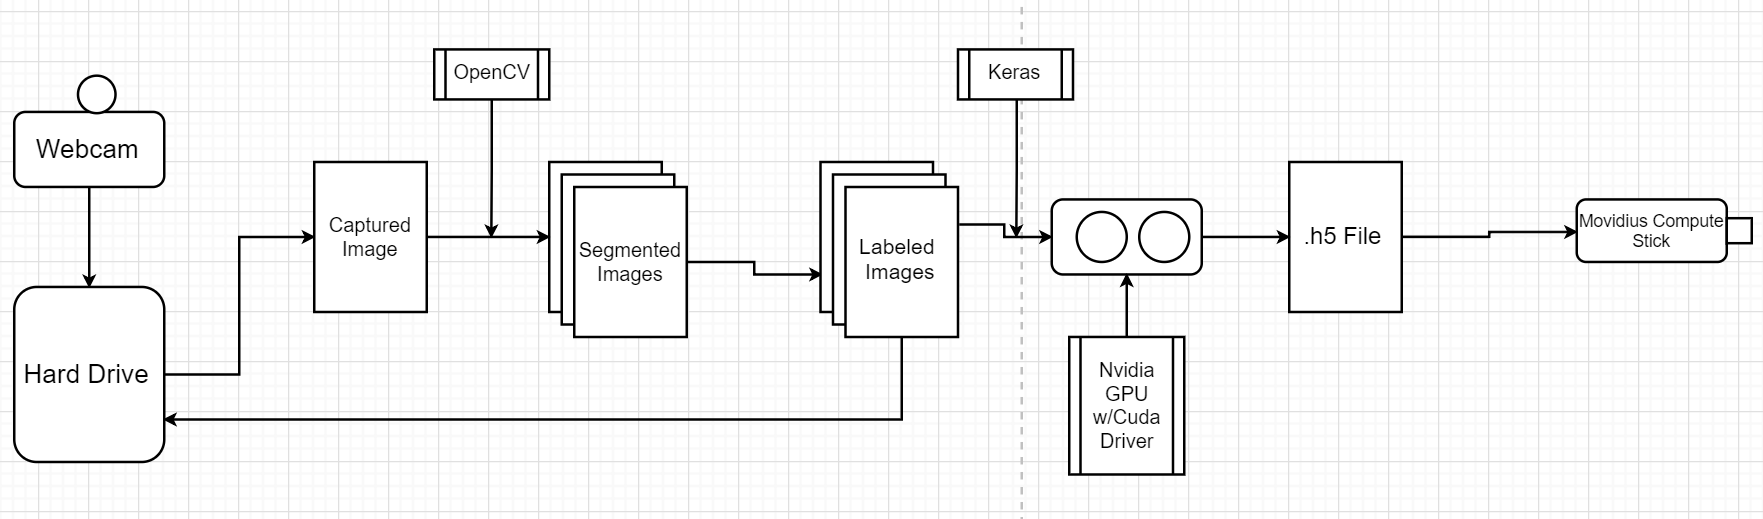
\includegraphics[height=6cm]{Trainingseeddiagram}
\end{figure}

The initial steps in our final product is similar to the training process. We start with the capturing of images and segment them in the same python script using opencv. The partitioned images with individual seeds are stored into a specified folder for classification. A separate python program will be developed with the .h5 file from the compute stick loaded to classify images fed through the hard drive, the output of the classification will be sent to two external sources. One, back to the hard drive with references to the images to be stored onto the database, two the output will be sent to another python program, that will invoke a system call to light up an LED if a bad seed is detected.

\begin{figure}[h]
\caption(Raspberry Pi Diagram)
\centering
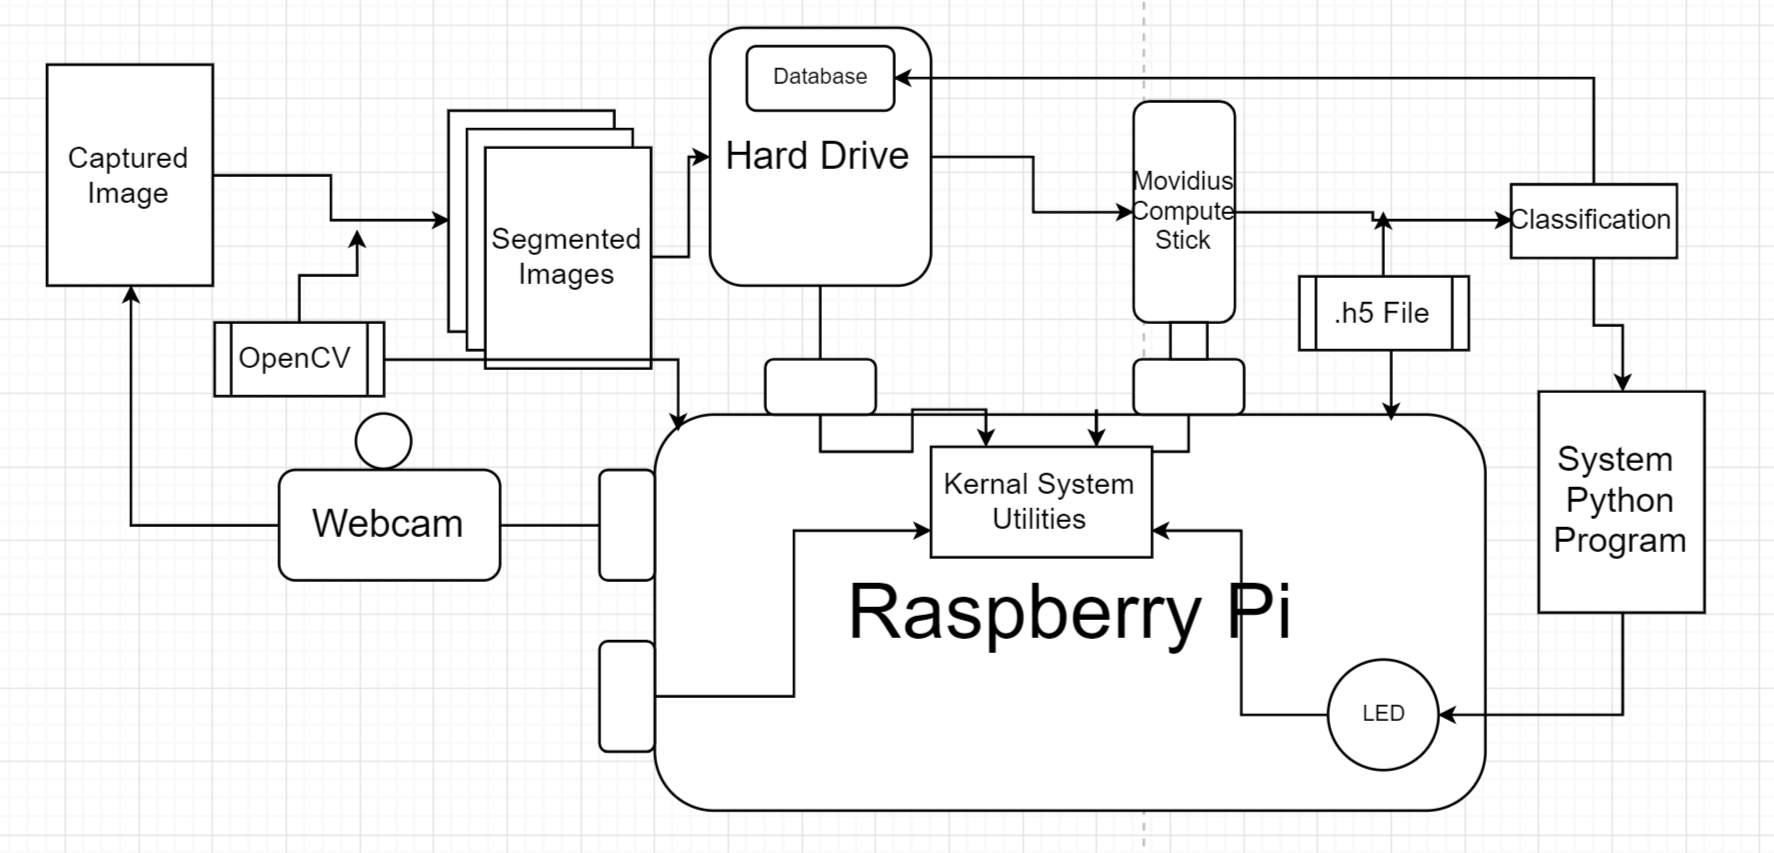
\includegraphics[height=6cm]{Raspiseeddiagram}
\end{figure}


\section{Database}

\subsection{Context}
The database exists to store the images used by the neural network, including training data, and data collected at runtime for future training and testing. 
Images will generally be added one at a time during runtime, but during testing and development the capability to add several, potentially hundreds of images per transaction. 

\subsection{Dependancies} 
The database will not depend on any other subsystem for opperation.

\subsection{Structure}
Making use of SQLite, the database itself will consist of a single file, alongside a folder containing the named image files. 
The database will consist of several tables, one for the training, one for verification, and one for images collected during runtime. 
The training table will consist of the following columns: index (integer), image address (String), actual type(boolean). 

\begin{figure}[h]
\caption{testing database example}
\centering
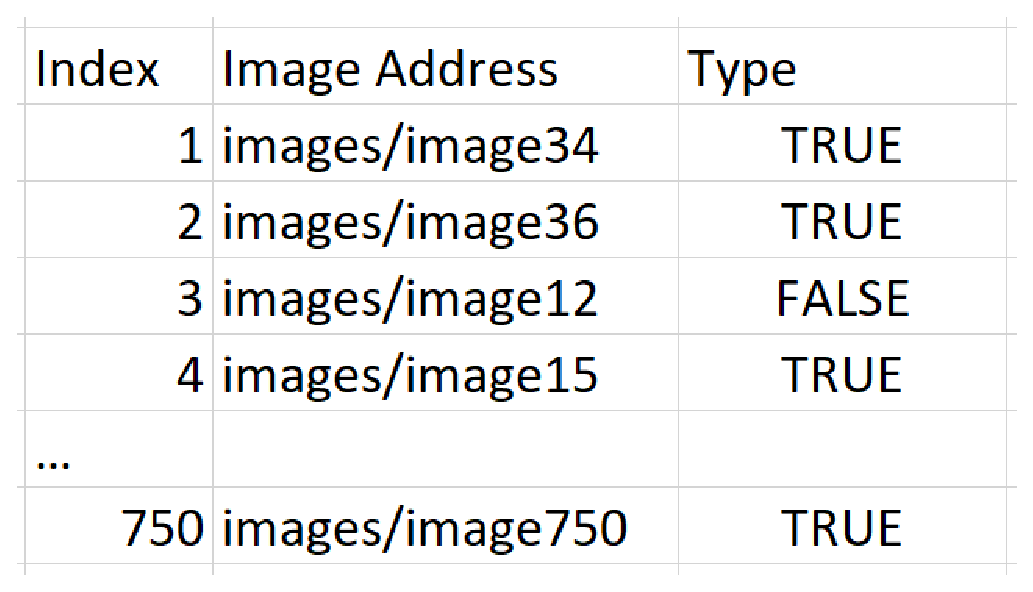
\includegraphics[height=4cm]{testingdb}
\end{figure}

The verification table will consist of the same columns with the addition of a flag column to indicate that during verification, the neural net missclassified the image in the entry. 

\begin{figure}[h]
\caption{verification database example}
\centering
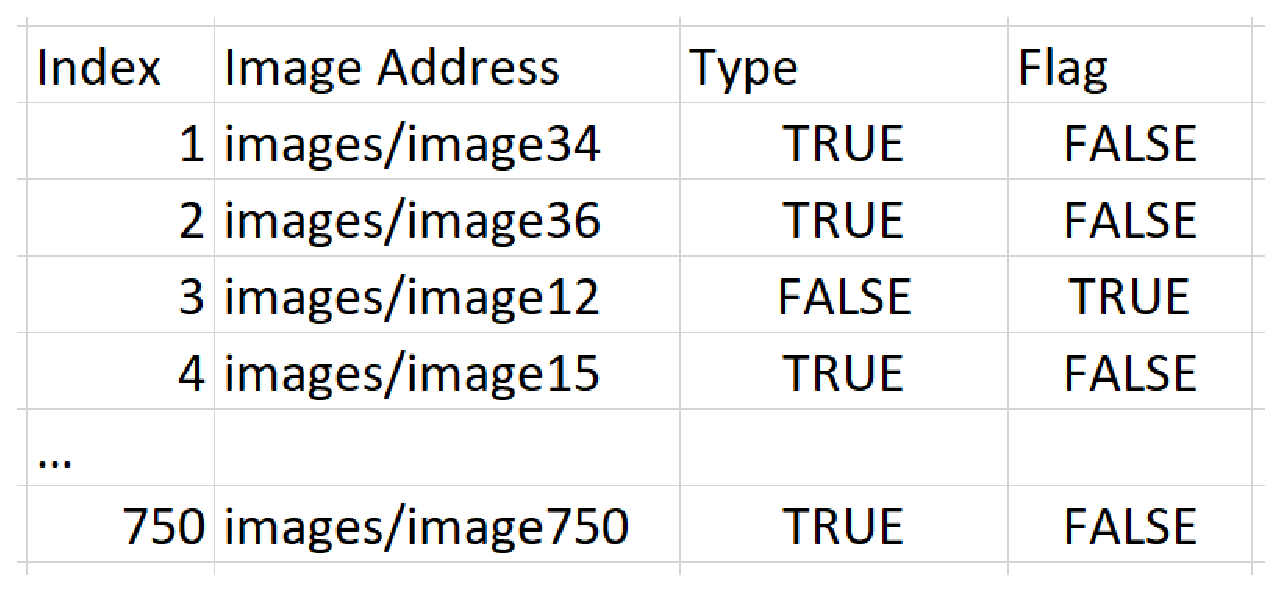
\includegraphics[height=4cm]{verificationdb}
\end{figure}


Finally the runtime table will consist of an index (integer), image address (String), and guess(boolean).

\begin{figure}[h]
\caption{runtime database example}
\centering
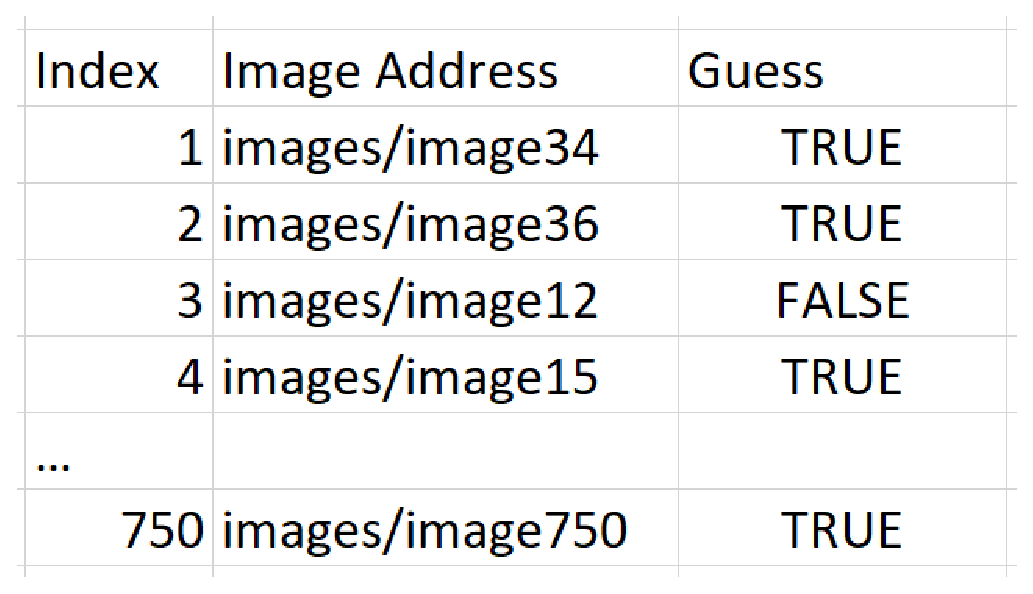
\includegraphics[height=4cm]{runtimedb}
\end{figure}

Each of these tables will share a database file, and a folder to store images in.
While not in use, this foder could be compressed into a tar archive, but would be uncompressed before runtime or during startup.




\subsection{Logical}

The database will be coded to support the following functions:

\begin{minted}{Python}

#returns the image address associated with the given the db index.
entry getImage(index, table);

#returns the image addresses associated with the given index range.
getImages(start, end, table);

#adds [num] entries to the db table.
void addImages(entries, int num, table);

#performs the given query, and returns an array containing the results.
query(query);

\end{minted}

The getImage, and getImages functions are designed to allow easy querying of images iteratively during neural network training. In such cases, we only care that each data point gets used, and filtering results based on type or guess is unlikely to be necessary.
The addImages function allows the system to add add the seed images collected during runtime to the database.
The query function allows us to move entrys to different table in order to increase the size of the training or verification data sets. 

\subsection{Interaction}

The database will interact with other subsystems by receiveing and servicing requests to access data in the database. During training, this will be returning entries from the training and verification data sets. At runtime, the system will present images to save via the addimages function. Each iteration, developers will utilize the query function to perform less typical opperations, including migrating runtime data into the training and verification tables.

\subsection{Resources}

The database will require little RAM, but will require its own drive in order to support storing a large number of images. We estimate that drive size will be close to 10 GB, but depending on the size of the training dataset, additional or less memory may be necessary.




\section{Neural Net}

\subsection{Context}
The specific structure of the human brain and eyes enable us to distinguish the things we see quickly. It is hard to make a software program to do the same thing by just using traditional programming methods. Neural networks solve this obstacle differently. The technique is to let the system through a training process with a large amount of experimental data to teach the neural network how to identify the target object. A critical component of the neural network is called perceptron. The perceptron absorbs multiple inputs and generates the result. For a perceptron, every input has a weight(threshold) that can represent the importance of that input to the output, and the perceptron can base on the weight to determine what the result will be. We can set different weights for input, then the decision-making models of perceptron will be different. What we just introduced is how a single perceptron works. If we connect multiple perceptrons, they will build a complex network of perceptron's that can make subtle decisions.  Each perceptron of the neural network only has one output, but the result is used as an input for many of other perceptrons. The weight or we can call it threshold condition judging is too heavy for the neural network system to do calculation; it will be better to use bias to simplify the notation of the condition. [1]

\subsection{Training}
Six types of artificial neural networks that are used in machine learning currently: radial basis functions neural networks, feedforward neural networks, recurrent neural networks, convolutional neural networks, Kohonen self-organizing neural networks, and modular neural networks. The neural network we introduced above is called feedforward neural network – artificial neuron, and we will use this specific neural network in our computer vision grass seed sorter project to identify seeds.  [2]
The neural network system requires clear and informative data to train.  We also need to initialize our weights randomly. There is a function called loss-function that is used to determine how good our neural network performs in a particular task. In the process of training, we start with a lousy performing neural network and end up with high accuracy. We keep adjusting weights to find a better performance than the initial one, so long as we have enough labeled examples for the network to learn from.  [3]
To training neural networks requires enormous computational power to deal with huge data set. Our university has 7 NVIDIA 1080Ti graphics cards, we may able to get access to them and use them to train our neural network. Since the project requirement asks the accuracy need to be at least 99.9 \%, we need at least 1000 images of each type of seed in order to achieve high accuracy of pure seed. To build our data set, we can get pictures from the previous team’s database. If the data from the previous team is not enough, we will take more images of each type of seeds to adjust the neural network to make it performs better.

\subsection{Framework}
We need to pick a framework to implement our neural network. The advantage of using a framework to create a neural network is that it can perform better and make neural network understandable and maintainable for others. Many choices are free online, such as Chainer, Gluon, Tensorflow, and PyTorch. The tool we decided to use to implement the neural network is called TensorFlow.
From the introduction of TensorFlow application, "TensorFlow is an open source software library for numerical computation using data flow graphs. Nodes in the graph represent mathematical operations, while graph edges represent multi-dimensional data arrays (aka tensors) communicated between them. The flexible architecture allows you to deploy computation to one or more CPUs or GPUs in a desktop, server, or mobile device with a single API." After we install TensorFlow in our system, we can use it to make a neural network model.   

\subsection{Process}
By using TensorFlow to train our neural network, there are basically 7 steps we need to follow: 1. Import the images of seeds dataset 2. Explore the data 3. Preprocess the data 4. Build the model (Setup the layers, compile the model) 5. Train model 6. Evaluate accuracy. To import dataset, we use TensorFlow import data and load the data from the database directly, the types of seeds should be labeled. To explore the data, we need to see how many images we have in the database and what is the resolution of each image. To preprocess the data, we need to verify that the data is in the correct format. To build the model, we need to set up the layers and compile the model. The first layer is to transform the images from 2d-array to 1 d-array, and other layers consisted of neurons. Then we compile the model. To compile the model, we need loss function, optimizer, and metrics. The loss function is to measure the accuracy of the model. Optimizer updates model base on the result from loss function. Metrics is used to observe the process of training and testing. After the model is built, we start to train the model. We import data input model, then the model will learn to associate images and labels. For example, the model will be able to decide the type of seed that in the image. To do evaluate accuracy test, we base on the performant of our model and give a test accuracy. [4]

\subsection{Referencess}
[1]
Nielsen, \& A., M. (1970, January 01). Neural Networks and Deep Learning. Retrieved from http://neuralnetworksanddeeplearning.com/chap1.html
[2]
Shaikh, F., \& Faizan. (2018, April 04). An Introduction to Implementing Neural Networks using TensorFlow. Retrieved from https://www.analyticsvidhya.com/blog/2016/10/an-introduction-to-implementing-neural-networks-using-tensorflow/
[3]
(2017, November 27). How do we 'train' neural networks ? – Towards Data Science. Retrieved from https://towardsdatascience.com/how-do-we-train-neural-networks-edd985562b73
[4]
Maladkar, K. (2018, November 20). 6 Types of Artificial Neural Networks Currently Being Used in ML. Retrieved from https://www.analyticsindiamag.com/6-types-of-artificial-neural-networks-currently-being-used-in-todays-technology/
[5]
Train your first neural network: Basic classification  |  TensorFlow. (n.d.). Retrieved from https://www.tensorflow.org/tutorials/keras/basic\_classification


\section{Camera}

\subsection{Context}

The camera subsystem is responisble for capturing images of seeds on the conveyor belt on a timed interval and sending the images to the rasberry pi for image processing. The camera subsystem needs to provide clear and quick images to the vision processing subsystem, so that the seeds captured by each image can be identified and classified by the image processing subsystem. 

\subsection{Composition}
This subsytem will make use of a camera, usb connector, image control program, and a constant light. The camera needs to take high quality images fast enough to capture 15 or more small grass seeds per second. The image control program will need to send a signal repeatedly with a set interval in order to capture the images at a speed that is effective and useful for our system. The usb connector will be used to send signals and data in and out of both the camera as well as the raspberry pi. These images will then be processed by a different subsystem. The constant light will need to provide a source of light to the conveyor belt so that the images used dont change even with outside sources of light.

\subsection{Structure}
In order to get high quality images the team decided that a resolution of 1920 x 1080 would be sufficient for high definition quality to determine good and bad seeds. For image speed the camera would need to run more than 10 frames per second and 30 frames per second will allow us to be well above what we need. The camera we decided to use for our project is the Logitech C920 Pro Webcam which is able to take images at 1920 x 1080 resolution as well as doing so at 30 frames per second. This camera also comes with mounts attached to it and the mount allows the camera lens to look up or down for adjusting. 

The next part of this component is the program that sends a take image signal to the camera and saves the image in a specified way. The program will use a timer to take an image, wait, then take another image, wait, repeat. This will allow for a controlled amount of images sent as well as capturing all the seeds that go by. 

The light that we have will need to be strong enough to reduce the effect of outside light sources that change throughout the day. Since the program could be running at any time, any outside variables need to be removed in order to get consistant and accurate results. The light would need to be mounted above the seeds near or next to the camera in order to reduce shadows. 

\subsection{Logical}
For the camera subsystem we will be using OpenCV, an open source vision software, in order to capture and analyse initial images. The program writen with OpenCV will send a call to the camera to take an image every interval of time. The interval that we use to take images will be faster than the processing subsystem that way it doesn't have to wait for a return signal to take the next image. This will streamline the image taking and updating process so that it is not dependent on the speed of the next subsystem.

\subsection{Interaction}
The camera control program will interact with the camera, the hard disk, and the image processing system. The way it interacts is by sending a signal to the camera, then saving the image back to the hard disk, and then the image processing system will take the image from the hard disk and process it. The control program will then continue to to send signals on the timed intervals.

\subsection{Resources}
The camera system requires only a small amount of processing and storage. It needs enough storage to save a single high definition image that the camera takes and processing power to conisitently send a signal to keep taking images. It also needs to use one usb port on the Raspberry pi to connect the camera.


\section{Vision Processing}


\subsection{Context}

The goal of the vision processing subsystem is to transform each image received by the camera, and tranform the result into several
individual images, one for each identified seed, so that the neural net can classify them. 
This system will be responsible for identifying each seed present on the received image,
and creating a smaller image containing just that seed for each of them.

\subsection{Composition} 

This system will be composed of a single algorithm, making use of the OpenCV image processing library.
By making use of OpenCV, the algorithm should be reduced to initial filtering, noise removal, and thresholding.

\subsection{Algorithm}
Filtering will take the initial image and create a boolean array to establish whether each pixel made it through the filter.
Since the background will be quite consistant, this filter should be easy to create, but will be more formally established during testing.
After filtering we remove noise removal, which can be accomplished easily using the openCV morphologyEx() MORPH_OPEN operation.
Finally, utilizing OpenCV's distanceTransform() and threshold() functions, we can ensure each identified block is seperate, and use OpenCV's connectedComponents() function to identify each block and its coordinates. With those coordinates we can easily create a smaller image containing a single seed based on the initial image.

\begin{minted}{python}


img = cv.imread('someimage.png')
gray = cv.cvtColor(img,cv.COLOR_BGR2GRAY)
ret, thresh = cv.threshold(gray,0,255,cv.THRESH_BINARY_INV+cv.THRESH_OTSU)
kernel = np.ones((3,3),np.uint8)
opening = cv.morphologyEx(thresh,cv.MORPH_OPEN,kernel, iterations = 2)
sure_bg = cv.dilate(opening,kernel,iterations=3)
dist_transform = cv.distanceTransform(opening,cv.DIST_L2,5)
ret, sure_fg = cv.threshold(dist_transform,0.7*dist_transform.max(),255,0)

ret, markers = cv.connectedComponents(sure_fg)
\end{minted}


\subsection{Logical}

The vision processing subsystem will have a single function facing the remainder of the project. 
This function will take a single image as a parameter, and return an array containing
a set of images, each with one of the seeds identified. 

\subsection{Dependancies} 

The vision processing subsystem will require image data recieved from the camera subsystem.

\subsection{Interactions}

The vision processing subsystem will interact with both the camera, and neural network subsystems. 
The vision processing system serves as the in between code necessary to translate the image received from the camera
into images that the neural network is capable of identifying.

\subsection{Resources} 

The vision processing subsystem will run on the rasberri pi, 
and requires no additionaly memory resources.





\section{User Interface}

\subsection{Context}

The user interace subsystem needs to be capable of starting and stopping the execution of the entire system, and will be responsible for displaying any error messages that may arrise during execution.
Because the scope of the interface is fairly minimal, we plan to implement it via the command line.

\subsection{Composition} 

The user interface will operate in its own thread, with the ability to start the main program. 
The user interface can then wait for further input, and set a flag telling the main thread to stop upon receiving a shutdown command.

\subsection{Interaction and Dependancies}

The user interface will primarily interact with the user, and the remainder of the program as a whole.
Users will be supplied error messages, and give commands, while the UI starts the system, and sets flags for the
system to respond to. The user interface will be necessary to start the system, and doesn't
depend on any of the other subsystems. 

\subsection{Rational}

A command line interface was choosen to minimize the amount of work required to get a functional prototype built.
Since so little user interaction is necessary, this should have minimal impact on the usability of the system as a whole.
By keeping user interactions in a seperate thread, we reduce the amount of time 
the main thread spends checking for input, 
which allows the system to be more efficient overall. 
 


\end{document}
